% Copyright (c)) 2014,2016 Casper Ti. Vecto
% Public domain
\chapter{系統需求分析}

透過特性要因分析可以將比特幣的交易监督系统大致分為四個主題,如圖\ref{fish1}所示,分別為信息安全技術、加密貨幣錢包、近場通訊技術以及數據庫。針對四項主軸,最為一個金流系統,信息安全是不可或缺的環節,著重於商家認證機制、用戶權力控管、身份識別管理、使用者訪問控制四個方向;本系統致力於奠定匿名對實名的加密貨幣系統,必須對區塊鏈技術、公鑰私鑰生成算法、點對點交易技術、錢包地址產出以及貨幣發行技術五個方向進行探討;在交易場景中,本系統採用近場通信技術,因此需要對商品RFID標籤建置、讀取商品RFID標籤以及Android Beam傳輸商品交易進行基礎的API調研;為了使的加密貨幣實名制的實現,數據庫必須存儲與政府和商家相關的信息。此時數據庫加密、個資去識別化安全以及數據庫連接便相當重要。
		\begin{figure}[!htbp]
			\centering
			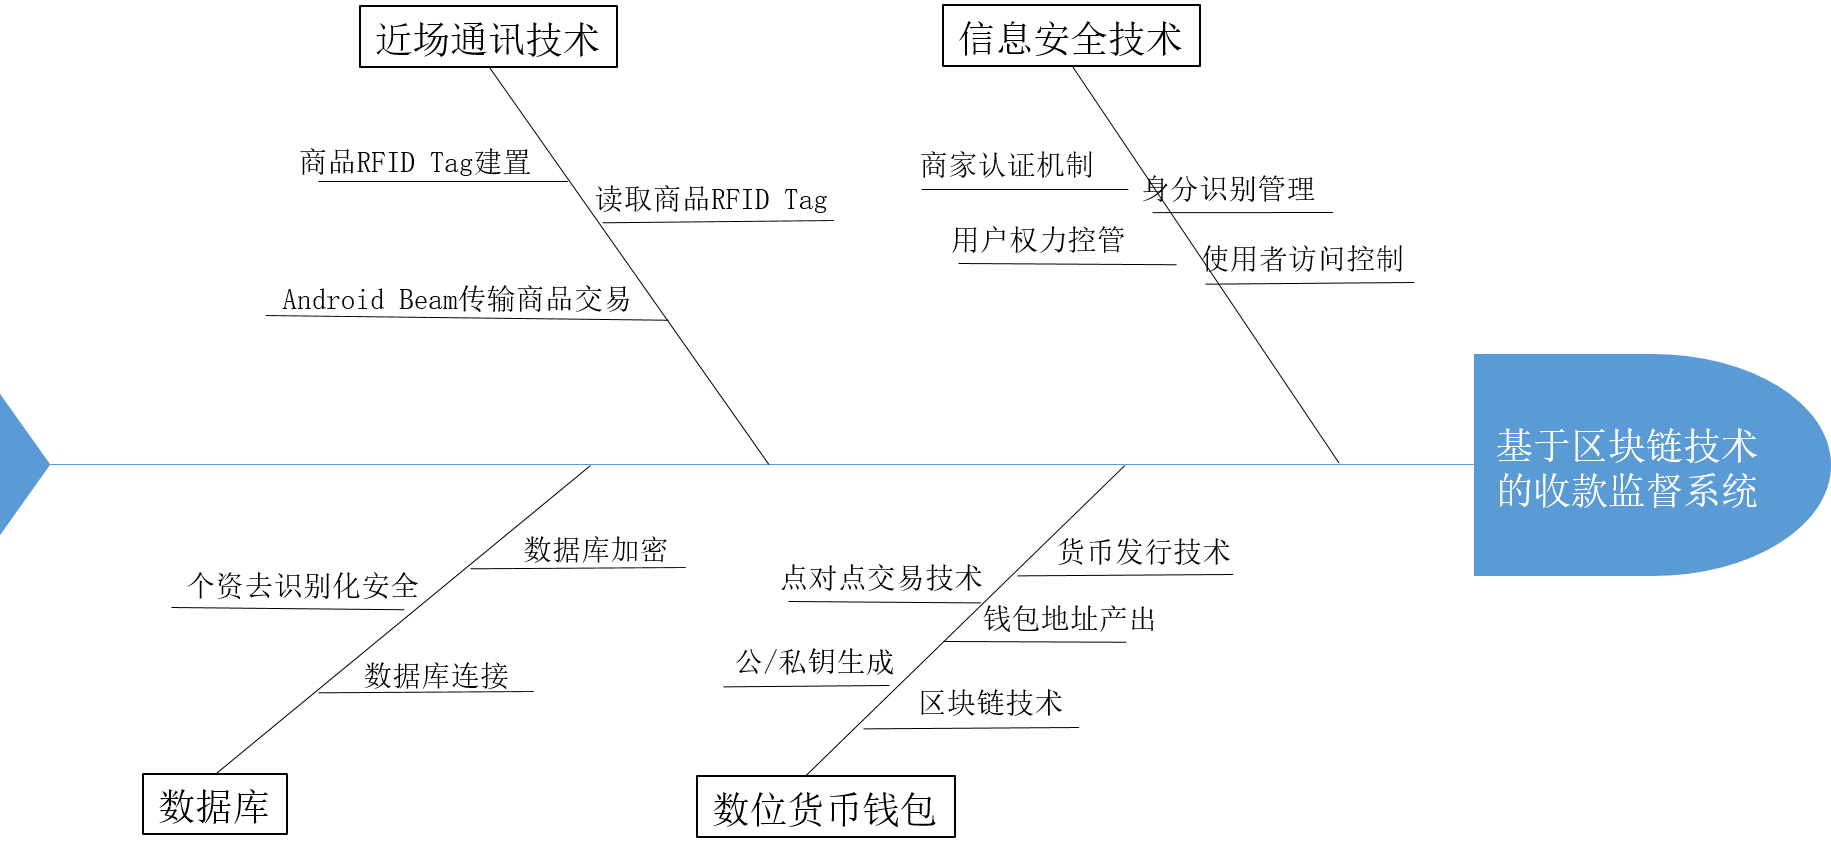
\includegraphics[width = 0.8\textwidth]{fish1.png}
			\caption{特性要因分析图}\label{fish1}
		\end{figure}

為了使得本文提出的系統設計的模塊更加的明確,對系統進行詳細的需求分席可以確立應確立的方向,在本章將分為三節進行分析分別為交易模型分析、功能性需求分析以及特性要因分析。


\section{交易模型分析}

在設計比特幣的监督系统之前必須針對現今社會中人與人之間的交易方式進行分析,在支付的方式大致分為現金交易以及電子支付。
%%fig allan
\begin{figure}[!htbp]
	\centering
	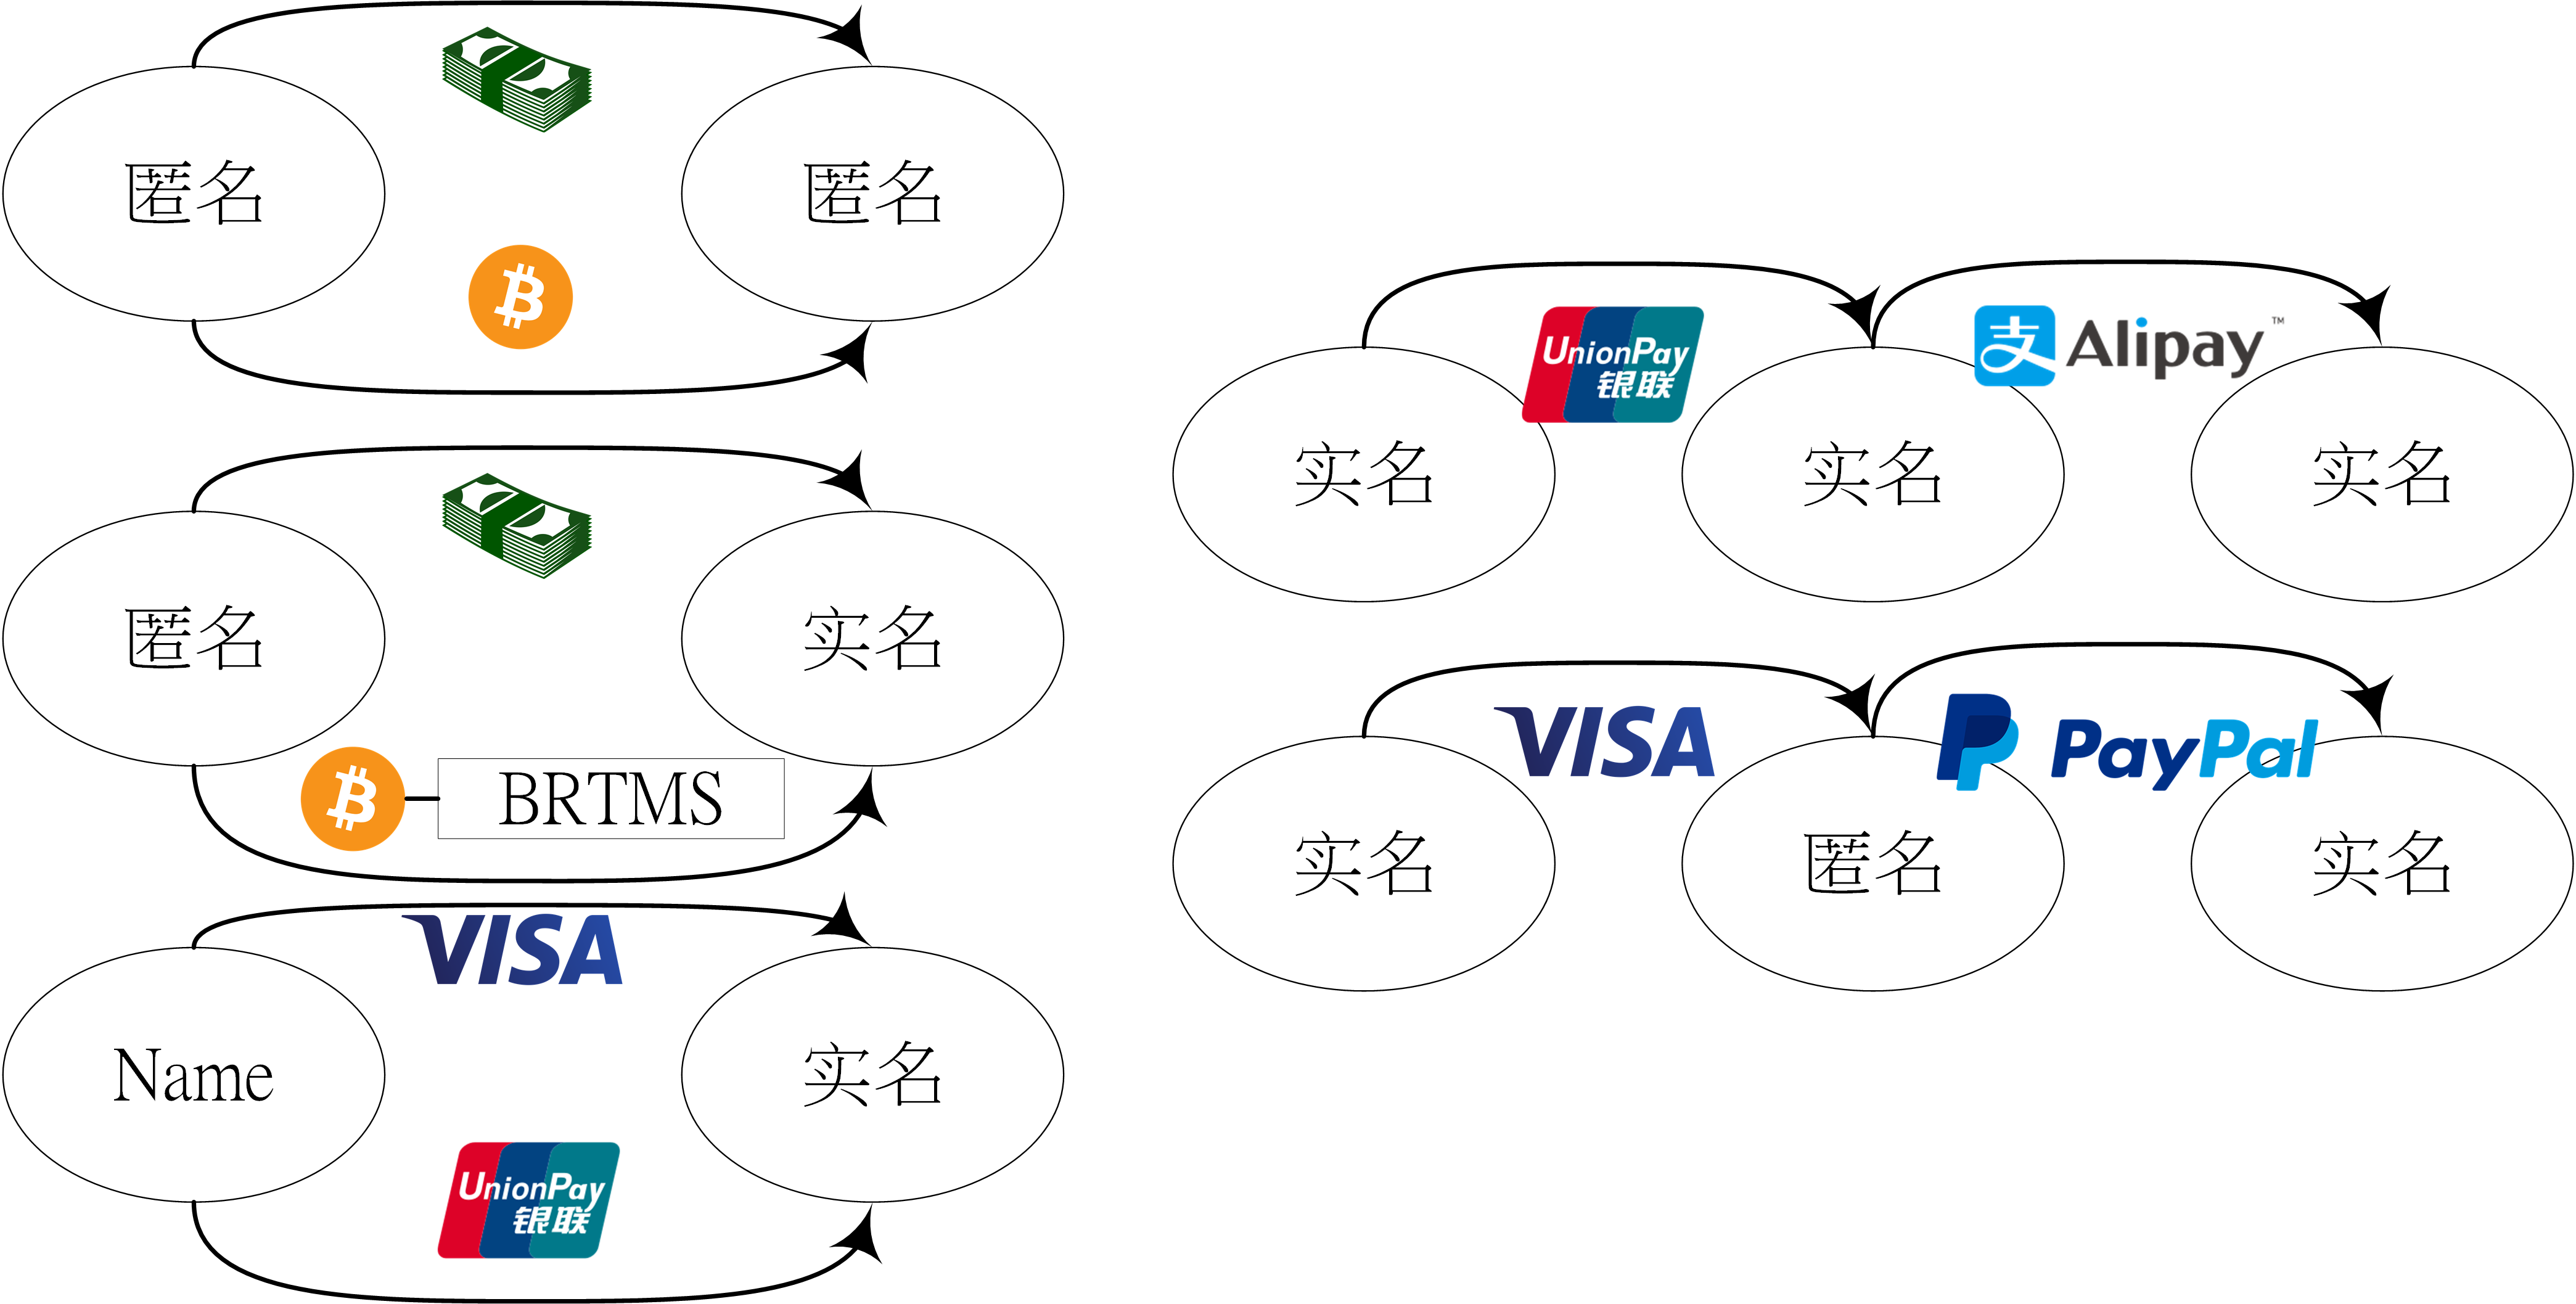
\includegraphics[width = 0.7\textwidth]{modeall.png}
	\caption{各種交易模型示意圖}\label{modeall}
\end{figure}

	\subsection{現金交易類型}
	在現金交易模型中大致分為匿名顧客支付匿名商家以及匿名顧客支付實名商家兩種,在過去的社會中,貝殼貨幣逐漸的被黃金取代,但黃金過於沈重在交易上相當不便。紙鈔的誕生漸漸地取代了黃金,也使得法定貨幣的誕生,法定貨幣包括鈔票以及錢幣,在過往的法定貨幣存在著黃金價值支撐,使得法幣具有價值,但經過歷史的變遷,法定貨幣漸漸地走向信用本位已無大量的黃進作為法幣的價值支撐。紙鈔以及銅幣的發行皆不帶有持有者的真實姓名,因此在現金交易模型分析中將顧客支付皆歸類為匿名支付,圖\ref{modeall}為各種交易模型示意圖。

		\subsubsection{(一)匿名顧客支付匿名商家交易模型}
		現金法定貨幣的本身不存在使用者信息以及交易信息現金是一種匿名的支付方式,早期有許多的商家並無向政府進行註冊,當顧客完成挑選商品進行結帳的同時,顧客只是將現金貨幣交付給商家,商家將商品賣給顧客,但在這過程中並無開立收據。在商家無開立收據的情況下,顧客完成此次的交易後,倘若該商品存在著瑕疵,進而引起商家與客戶之間的消費糾紛,這使得在追根究底的過程中存在的沒有憑據的困擾。對於顧客匿名支付匿名商家可以保有顧客的信息隱私,但無法保障顧客應有的顧客權益。商家在未開立收據的同時可以避開政府的稅收,這使得政府在課徵稅收的過程變得困難,且商家所販售的商品並無得到明確的信息紀錄,對於商家庫存管理只能依靠過去的經驗。政府而言,商家販售的商品並無完整的商品信息,無法對商家商品進行安全性檢驗,使得國民購買的商品存在的許多安全疑慮。

		\subsubsection{(二)匿名顧客支付實名商家交易模型}
		現今最為常見的交易模式為匿名顧客支付給實名商家,在顧客以匿名現金法定貨幣進行交易時,商家只要開立收據,即被歸類為匿名顧客支付實名商家交易模型。商家在開立收據的同時,在收據上記載的信息包括職工號、商家信息以及產品信息。記錄職工信息為了確立該筆交易應該賦予責任的人員,商家信息使得當顧客與商家發生交易糾紛時可以尋得取得賠償的對象,產品信息詳細記載顧客於該商家購買的商品。對於顧客,基於現金法定貨幣的匿名使顧客依舊保有顧客信息隱私,但卻因為商家開立收據可以保障顧客權益。商家因為開立收據使得商家為實名,因為實名使的商家可以可以經營品牌形象,除此之外,因為收據紀錄了產品信息這讓商家在庫存管理以及收入計算變得更加容易。對政府而言,可以檢視商家的所得以及商家販售的商品,使政府可以更有效率的課徵稅收以及檢驗管理產品安全。

	\subsection{電子支付類型}
	電子商務的日趨盛行電子支付交易模型也日漸普及,電子支付與加密貨幣的區塊鏈技術不同的是採用數據庫存儲著所有的交易信息,而用戶要能夠使用電子支付也必須接受電子支付運營商實名制的條件。在電子支付的數據庫中存在著黑客攻擊、信息不一致以及中心化運營的風險,但電子支付有效解決了遠距離支付的瓶頸,也使得現今的網路購物變得更加的方便。在電子支付交易模型中分為三種交易分別為實名顧客支付實名商家、實名顧客透過實名第三方再實名商家以及實名顧客透過匿名第三方再實名商家,以下將逐一說明。

		\subsubsection{(一)實名顧客支付實名商家交易模型}
		VISA為國際電子支付公司在在申辦VISA電子支付前必須做詳盡的身份認證,VISA電子支付為中心化的運營,使得公司可以凍結相關用戶的戶頭以及得到所有的用戶信息,且為了保護顧客隱私所有的交易信息皆存儲在VISA公司的數據庫當中。VISA公司透過不斷的優化電子支付技術已經可以接受每秒兩千筆的交易,為了使得VISA公司能夠穩定的運營電子支付服務,VISA公司將收取每筆交易固定比例的手續費。再透過VISA電子支付的過程中,顧客因為必須進行實名驗證,使得顧客必須透露顧客個人信息,甚至可以針對這些個人信息進行商業上的交易。對於商家必須承擔VISA電子支付所需的手續費,使得商家商品價格必須做出相對應的調整,對政府而言,因為交易信息皆以中心化的方式存儲,可以更方便的檢視,且可以更快速的查閱商家的收入課徵應繳的稅收。
		

		\subsubsection{(二)實名顧客透過實名第三方支付實名商家交易模型}
		電子支付的方式日趨普及也使得可選擇的電子支付的渠道更加多元,較為常見的包括VISA電子支付以及銀聯電子支付,而每一家銀行為了使得顧客於電子商務的支付上更為便利會同時選擇電子支付,使得銀行卡支持電子支付,但多加的銀行卡林立使得顧客在卡片管理上更加的繁瑣,屆時但三方的整合平台變成為解決方案。顧客可以在實名第三方支付添加多張卡片,再以第三方支付進行付款。實名顧客透過實名第三方支付實名商家,顧客可以得到更方便的銀行卡管理,但卻在第三方支付上透露了個人交易信息,對於商家可以僅支持第三方支付卻同時接受多家不同銀行卡的支付方式,對於政府僅需要調閱第三方支付公司僅可查閱該故可的所有用戶的交易信息,且可更完整的採集到商家的收入信息。
		
		\subsubsection{(三)實名顧客透過匿名第三方支付實名商家交易模型}
		為了使得顧客可以保有更多的顧客隱私,Paypal提出了實名顧客透過匿名第三方支付實名商家的模型,顧客預支付一筆資金給商家,首先使用VISA支付一筆資金到Paypal公司,屆時Paypal公司將以公司本身的名義支付該筆款項,換言之,商家不會取得顧客相關的個人信息,也無法對顧客交易信息進行數據挖掘,值得一提的是,透過VISA支付可直接將資金直接支付給商家但必須支付小額的手續費,透過Paypal支付資金必須多經過一家公司,這使得交易手續費更加的昂貴,但也因為多一個程序的資金轉移,使得顧客的個人信息可以得到隱匿。實名顧客透過匿名第三方支付實名商家的交易模型,對顧客而言商家可以開立收據使得顧客保有顧客權益,同時也保有顧客的匿名性,但缺點是必須承擔高額的手續費。對於商家,可以透過交易信息管理商品庫存,快速的計算商家的收益。政府可以快速地檢視商家交易信息以及商家所得。

		\subsection{交易比較}
		在上述五大模型中可以看出,在初始的交易模型為匿名顧客支付匿名商家交易模型,但因為無法保障故可與商家的權益發展出匿名顧客支付實名商家交易模型這使得顧客與商家可以兼顧雙方權益,且可以讓政府快速地檢視稅務相關信息。因為支付技術的日新月異開始有了VISA電子支付,使得電子商務可以快速的運行,但因為VISA支付透露了太多的個人信息,因為顧客需求逐步推出以實名顧客透過匿名第三方支付實名商家交易模型為基礎的支付方式,兼具以以電子支付作為付款方式,卻同時保有個人隱私。但為一個缺點是需要多經過一個資經轉移的程序,造成手續費為多種交易模型中最為昂貴。有上述分析可知,現金法定貨幣最佳的交易模型為匿名顧客支付實名商家交易模型,而電子支付類型的交易模型演變也是往同一方向演進。
		在加密貨幣支付中,大部分的交易皆為現金交易類型中的匿名顧客支付匿名商家交易模型,商家與顧客交易的過程中並無開立收據,使得顧客與商家發生消費糾紛時並無太多的依據。本文致力於使的加密貨幣可以同時兼顧顧客隱私且具有顧客權益,對於商家不需要支付手續費給運營商,且可以公開匿名的方式檢視所有的交易信息,使得政府在課徵稅收的業務上可以更加便利,表\ref{txvs}為交易關係比較表。


		\begin{table}[!htbp]
		\centering
		\caption{交易關係比較表}
		\label{txvs}
		\begin{tabular}{|l|l|l|l|l|}
		\hline
		 & 顧客 & 仲介單位 & 商家 & 商品 \\ \hline
		現金 & 匿名 & 無 & 匿名/實名 & 匿名/實名 \\ \hline
		VISA & 實名 & 無 & 實名 & 實名 \\ \hline
		支付寶 & 實名 & 實名 & 實名 & 實名 \\ \hline
		PayPal & 實名 & 匿名 & 實名 & 實名 \\ \hline
		加密貨幣 & 匿名 & 無 & 匿名/實名 & 匿名/實名 \\ \hline
		\end{tabular}
		\end{table}

\section{功能性需求分析}

在現今的比特幣交易系統中為匿名對匿名支付的交易模式,這樣的交易模式無法保障顧客權益,也使得政府無法再加密貨幣交易當中課徵稅收。在傳統的支付系統當中是實名支付給實名的交易模型,雖然可以有效地保障顧客權益,且使得政府可以課徵稅收,但在這對顧客個人隱私日趨重視的世代中,個人信息越來越有價值,個人信息的保護更是成為重要的課題。在本系統中,將以加密貨幣比特幣為基礎,設計一個以匿名顧客支付給實名商家為基礎的系統,在實現匿名支付給實名的交易模型的同時,也將商家的庫存信息同時加入,使得商家可以簡單的在本系統中管理商家產品庫存。在本系統中如圖\ref{UC}參與者總共有三種分別為商家、職工以及顧客。以下將逐一說明:

商家,在本系統中第一個參與者,因為必須要有商家的註冊參與,才可以進一步的添加職工以及商家產品信息,如此一來商家才有商品可以販售。參與者商家本身有三項需求,分別為用戶註冊與登入、職工管理以及商家產品管理:

	\begin{enumerate}
	\item 用戶註冊與登入:為了得到政府的認證,商家必須接受政府的檢視,提交相關的信息到本系統中。在用戶註冊的頁面當中,進行用戶的註冊或是登入都需要用戶信息,因此需要包括加載用戶信息。
	\item 職工管理:在完成用戶註冊與登入之後,才得以進行職工管理,商家本身會有大於或等於一個職工的帳號,商家的註冊者本身會是一個職工。在職工管理當中,需要有修改職工帳戶與查詢職工帳戶兩項功能,查詢職工帳戶的功能必須包括加載職工信息。在進行職工帳戶修改時需要包括職工信息以及商家信息,才得以對職工信息進行修改。
	\item 商家產品管理:商家需要添加產品信息至商家產品信息中,產品為政府認可的產品認證編號,在本系統中產品本身不存在價格,需要參與者商家將產品添加至商家產品信息中才可以添加價格,這樣的設計可以使得在不同的商家可以設置不同的價格。除了商家對商家產品價格需求,同時也需要對產品庫存進行管理,透過區塊鏈加密貨幣公開交易信息的特性,可以使得庫存管理以及交易信息更快速地核對。在商家產品管理中需要查詢產品信息,在查詢產品信息的同時包括加載產品信息,使得查詢過程可以順利運作。在查詢完成產品信息後,商家需要將產品信息與商家信息添加到商家產品信息當中,在這過程中需要包括加載商家信息以及商家產品信息。

	\end{enumerate}

職工,需要進行用戶註冊並且通過政府的審查,在完成政府的審查之後需要進入商家交易管理建置移動收銀機:

	\begin{enumerate}
	\item 用戶註冊與登入:要成為職工之前職工需要進行用戶註冊,等待政府的審查之後,並經由商家進行職工管理將用戶與商家一併提交到職工信息,才得以成為正式的職工,職工的用戶註冊與登入皆需要包括加載用戶信息,才能使得註冊與登入功能順利運行。
	\item 商家交易管理:在完成登入後,商家交易管理將會加載相關信息,包括加載職工信息,在交易信息中添加職工編號,加載商家信息使得在進行交易的過程中可以將商家的比特幣地址傳送給顧客等待接收款項以及加載商家產品信息使得職工的移動設備上可以顯示所有的商家產品信息,在完成信息加載後職工的移動裝置已經成為一台移動收銀機。在職工在進行掃碼的過程會創建交易清單並且將交易清單傳送給顧客等待顧客的付款。在等待付款時,商家交易管理需要認證該筆交易是否有效,因此需要加載交易信息,
	\end{enumerate}

顧客,為了保持顧客的身份匿名,參與者顧客與參與者職工和商家不同,顧客在參與本系統的同時不需要註冊帳戶以及登入用戶帳戶,顧客主要需求為加載過去與顧客相關的交易信息,以及使用比特幣支付進行付款:
	\begin{enumerate}
	\item 顧客交易管理:顧客需要加載交易信息,但因為交易信息中的信息並無詳細闡述商家產品信息,因此需要進一步加載商家產品信息使得交易明細更加的清楚。除了顯示過去的交易信息的需求,顧客更需要創建一筆交易進行比特幣付款。付款完成之後,等待參與者商家向顧客說支付完成即可。
	\end{enumerate}

	\begin{figure}[!htbp]
	\centering
	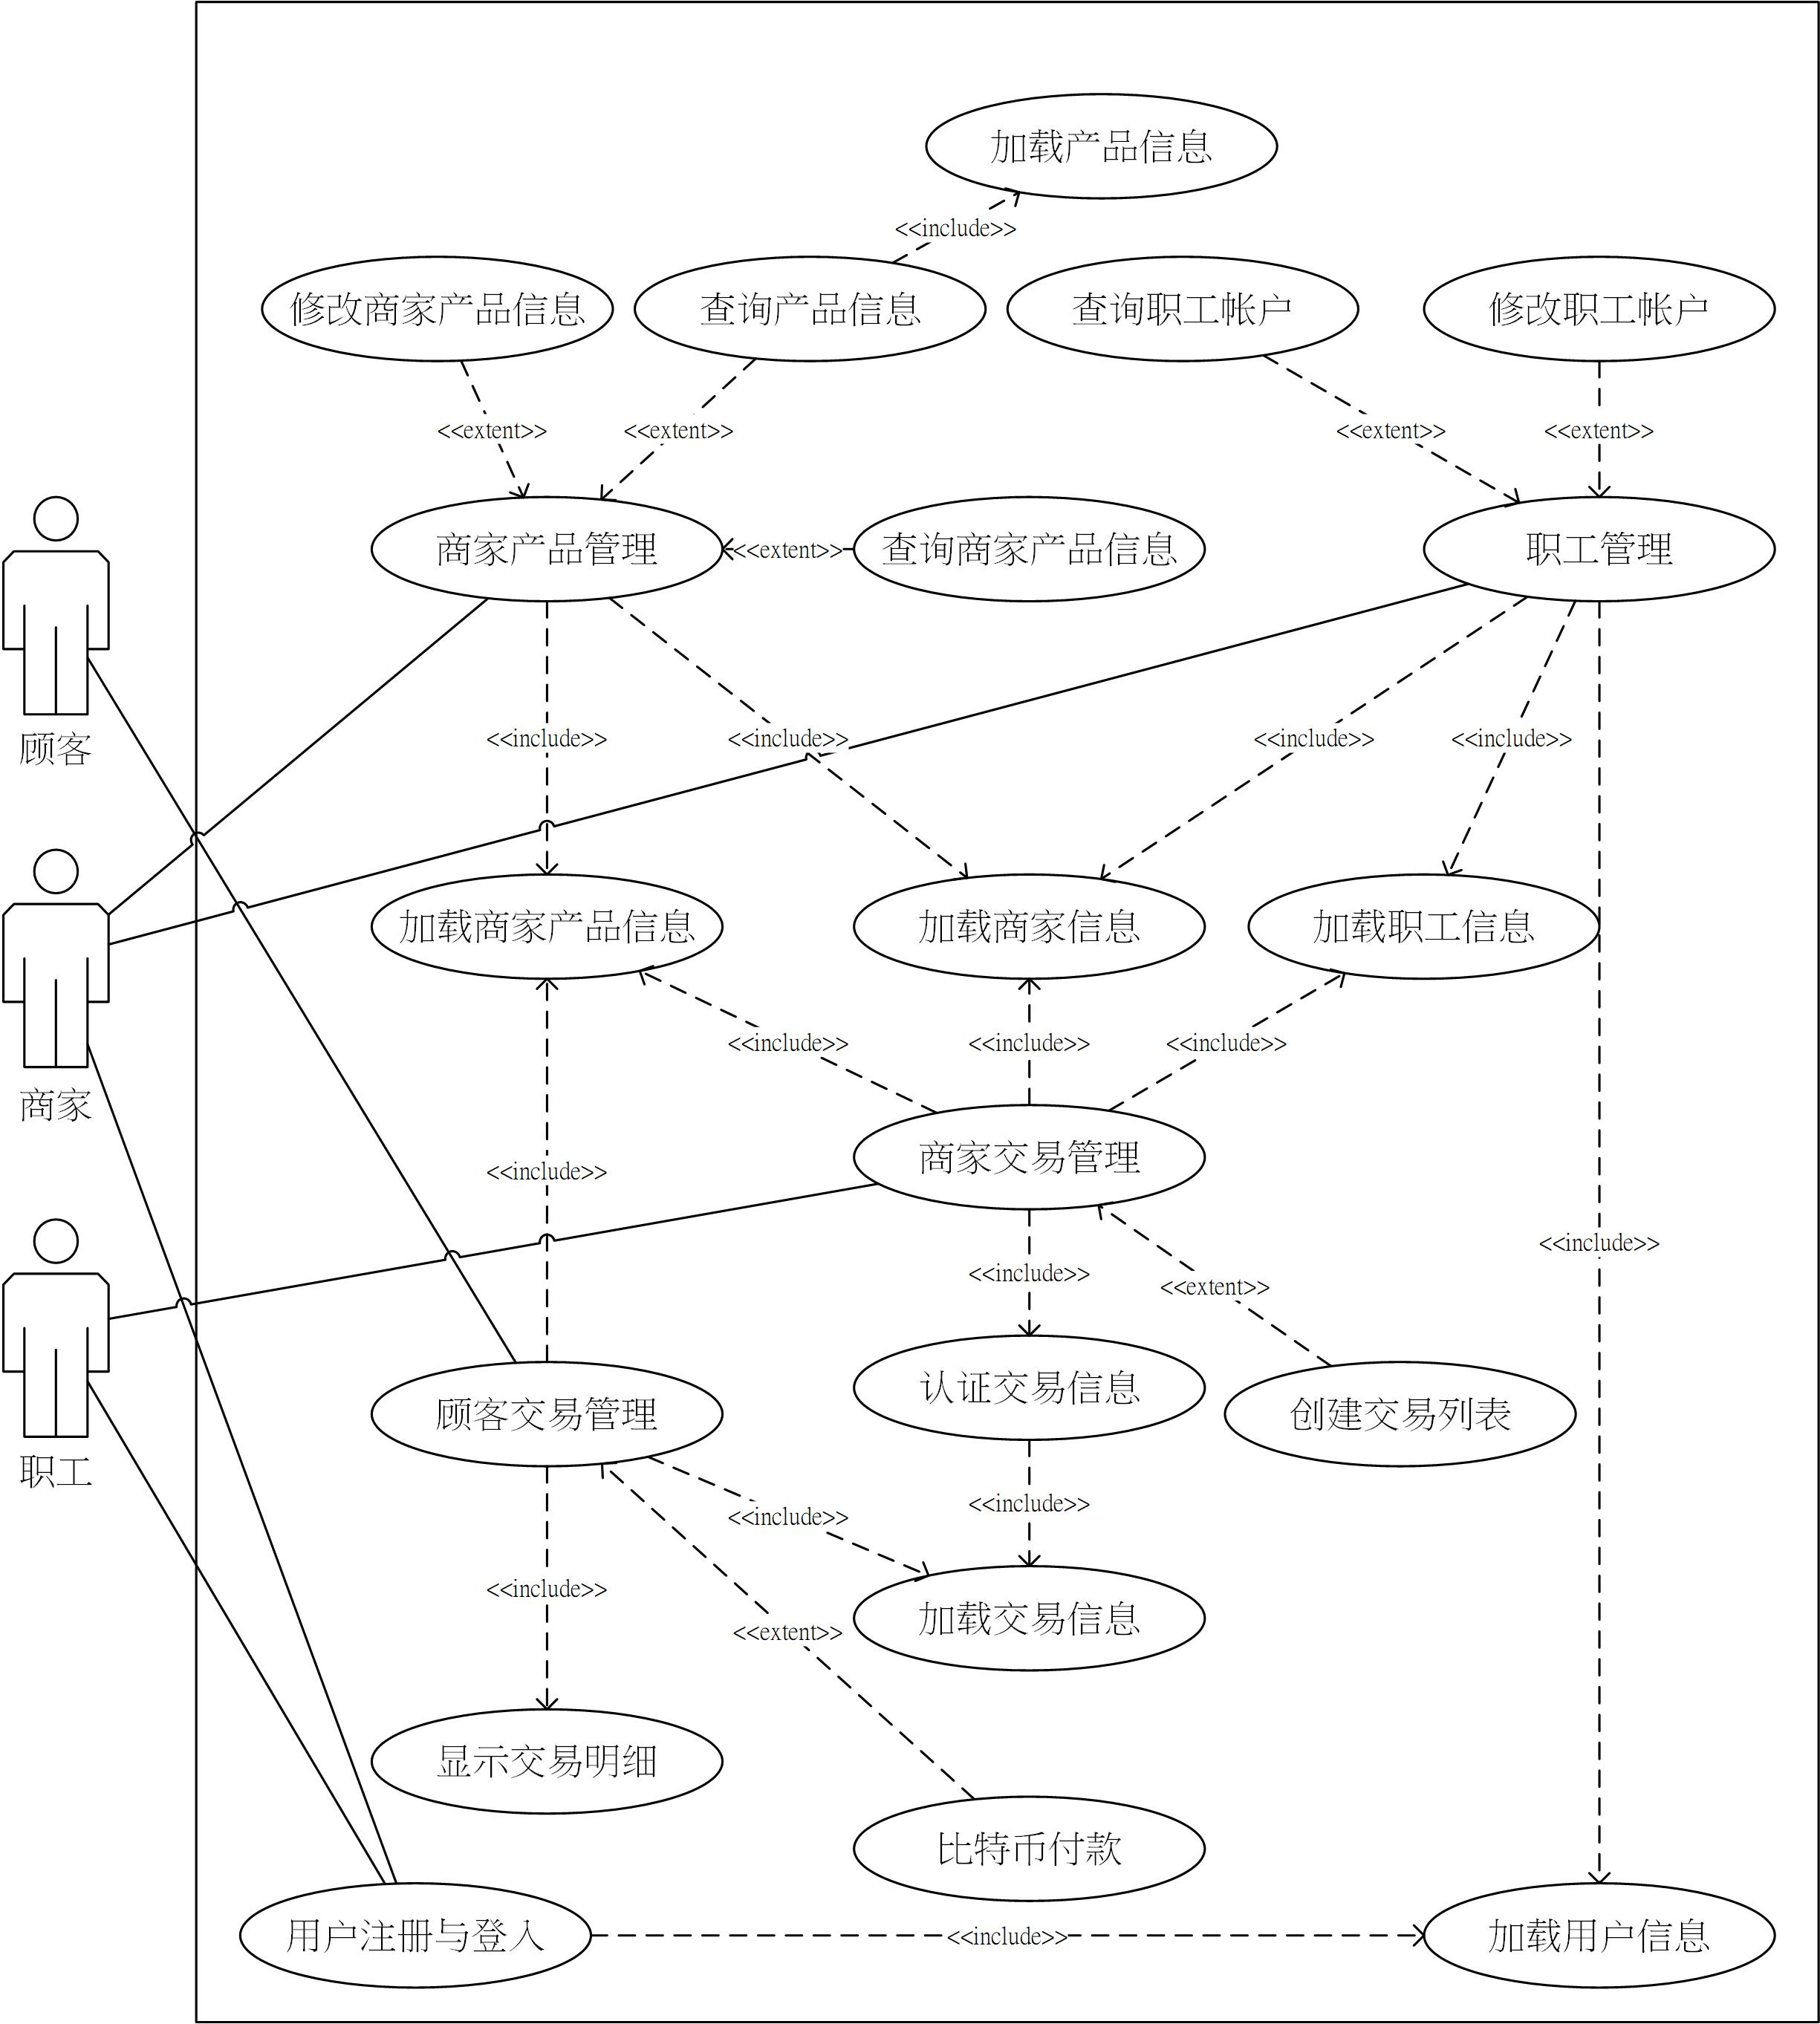
\includegraphics[width = 0.9\textwidth]{UC.jpg}
	\caption{系統用例圖}\label{UC}
	\end{figure}

	\section{非功能性需求分析}

	\subsubsection{(一)性能需求}
	
	本文所實踐之系統為比特幣的交易监督系统,參與者商家需要使用到商家端建置與管理商品資訊子系統,在參與者商家操作該子系統時,系統在設置完成後,於存儲的過程中應於三秒內完成。於商家端建置與管理商品資訊子系統、商家端行動收銀與交易明細系統應達到於兩秒內完成完成子系統與數據庫之間的信息傳遞以及信息存儲,倘若商家與顧客在完成交易後,卻無法得到快速的系統響應,這使得參與者顧客與職工遲遲無法離開收銀,甚至導致商家的交易塞車影響用戶的消費體驗。

	\subsubsection{(二)可拓展性}

	本論文提出的系統為比特幣的交易监督系统雛形,於系統設計中將考慮最為最必要的功能加以實現,包括商家端建置與管理商品資訊子系統、商家端行動收銀與交易明細系統以及顧客端行動支付與交易明細系統,於上述三個子系統中皆可以進行數據庫欄位的添加,使得交易信息、商家信息、商品信息、商家產品信息、用戶信息以及職工信息更加的完備且更符合實際上業務需求。在未來甚至可以加入更完整的稅務信息,使得政府在於稅務計算方面可以更加地減少人力資源的支出且更快速地進行統計,於庫存管理方面可以加入庫存預測的服務。

	\subsubsection{(三)可操作性}
	在本系統中的三個子系統中商家端行動收銀與交易明細系統以及顧客端行動支付與交易明細系統為實現在手持移動裝置Android操作系統上,於介面設計方面應給予商家用戶以及顧客用戶人性化的操作交互設計,以及於代碼撰寫方面應更加簡潔,使得用戶再啟動本手持移動端應用程序時可以在最短的時間內完成初始化程序加載,除了針對用戶交互方面的優化,也需要添加各個功能項目的使用說明以及用戶操作問題反饋,使得本系統的於移動設備的應用程序能夠儘速的修正提升用戶體驗。商家端建置與管理商品資訊子系統是以Java編程語言實現,針對參與者商家操作進行設計,該子系統需簡單明確的呈現商家信息、產品信息以及商家產品信息,使得用戶可以快速檢視所有商品,並新增、修改以及刪除該商家的相關產品信息,包括價格、庫存以商家產品描述。


	\subsubsection{(四)軟件與硬件環境需求}
	表\ref{eva}為本文提出系統的軟件與硬件環境需求,商家交易客戶端與顧客交易客戶端是建置在Android手機的應用程序,本文提出的交易方式為比特幣,因此導入bitcoinj\supercite{Bitcoinclients}對比特幣錢包進行管理,該套件可以生成比特幣地址、同步比特幣區塊鏈、透過AES加密算法保護比特幣錢包以及發起比特幣交易至比特幣網路。針對數據庫的控制數據傳輸選用JDBC\supercite{JDBCdatabaseaccesswithJava:atutorialandannotatedreference}實現數據庫的新增、修改、刪除以及查詢的功能,商家交易客戶端與顧客交易客戶端的手機移動裝置必須要內置NFC傳感器用來傳送與接收交易信息。商家管理客戶端是以Java編程語言實現軟件環境中需支持Java工作環境,服務器端需要SQL環境逕行數據庫搭建。


	\begin{table}[!htbp]
	\centering
	\caption{環境需求表}
	\label{eva}
	\begin{tabular}{|c|c|c|c|}
	\hline
	- & 操作系統 & 軟件 & 硬件 \\ \hline
	\begin{tabular}[c]{@{}c@{}}商家交易\\ 客戶端\\ 與\\ 顧客交易\\ 客戶端\end{tabular} & \begin{tabular}[c]{@{}c@{}}Android 4 \\ 或以上\end{tabular} & \begin{tabular}[c]{@{}c@{}}Java 7 或以上 \\ bitcoinjv0.14.6 \\ JDBC 4.2 或以上\\  Maven 3+\end{tabular} & \begin{tabular}[c]{@{}c@{}}存儲容量:32GB\\ 內存容量:2GB\\ 網路需求:10兆或以上\\ 傳感器:NFC傳感器\end{tabular} \\ \hline
	\begin{tabular}[c]{@{}c@{}}商家管理\\ 客戶端\end{tabular} & \begin{tabular}[c]{@{}c@{}}Windows 7 \\ 或以上\end{tabular} & \begin{tabular}[c]{@{}c@{}}Java 7 或以上 \\ JDBC\end{tabular} & \begin{tabular}[c]{@{}c@{}}硬盤容量:100GB\\ 內存容量:4GB\\ 處理器:Core 2 Duo 或以上\\ 網路需求:10兆或以上\end{tabular} \\ \hline
	服務器端 & \begin{tabular}[c]{@{}c@{}}Windows Server \\ 2003 \\ 或以上\end{tabular} & \begin{tabular}[c]{@{}c@{}}Microsoft SQL Server \\ bitcoin-qt 0.8.X 或以上 \\ Apache HTTP Server\end{tabular} & \begin{tabular}[c]{@{}c@{}}硬盤容量:1000GB\\ 內存容量:16GB\\ 處理器:Xeon E3 或以上\\ 網路需求:100兆或以上\end{tabular} \\ \hline
	\end{tabular}
	\end{table}




%		\begin{figure}[!htbp]
%			\centering
%			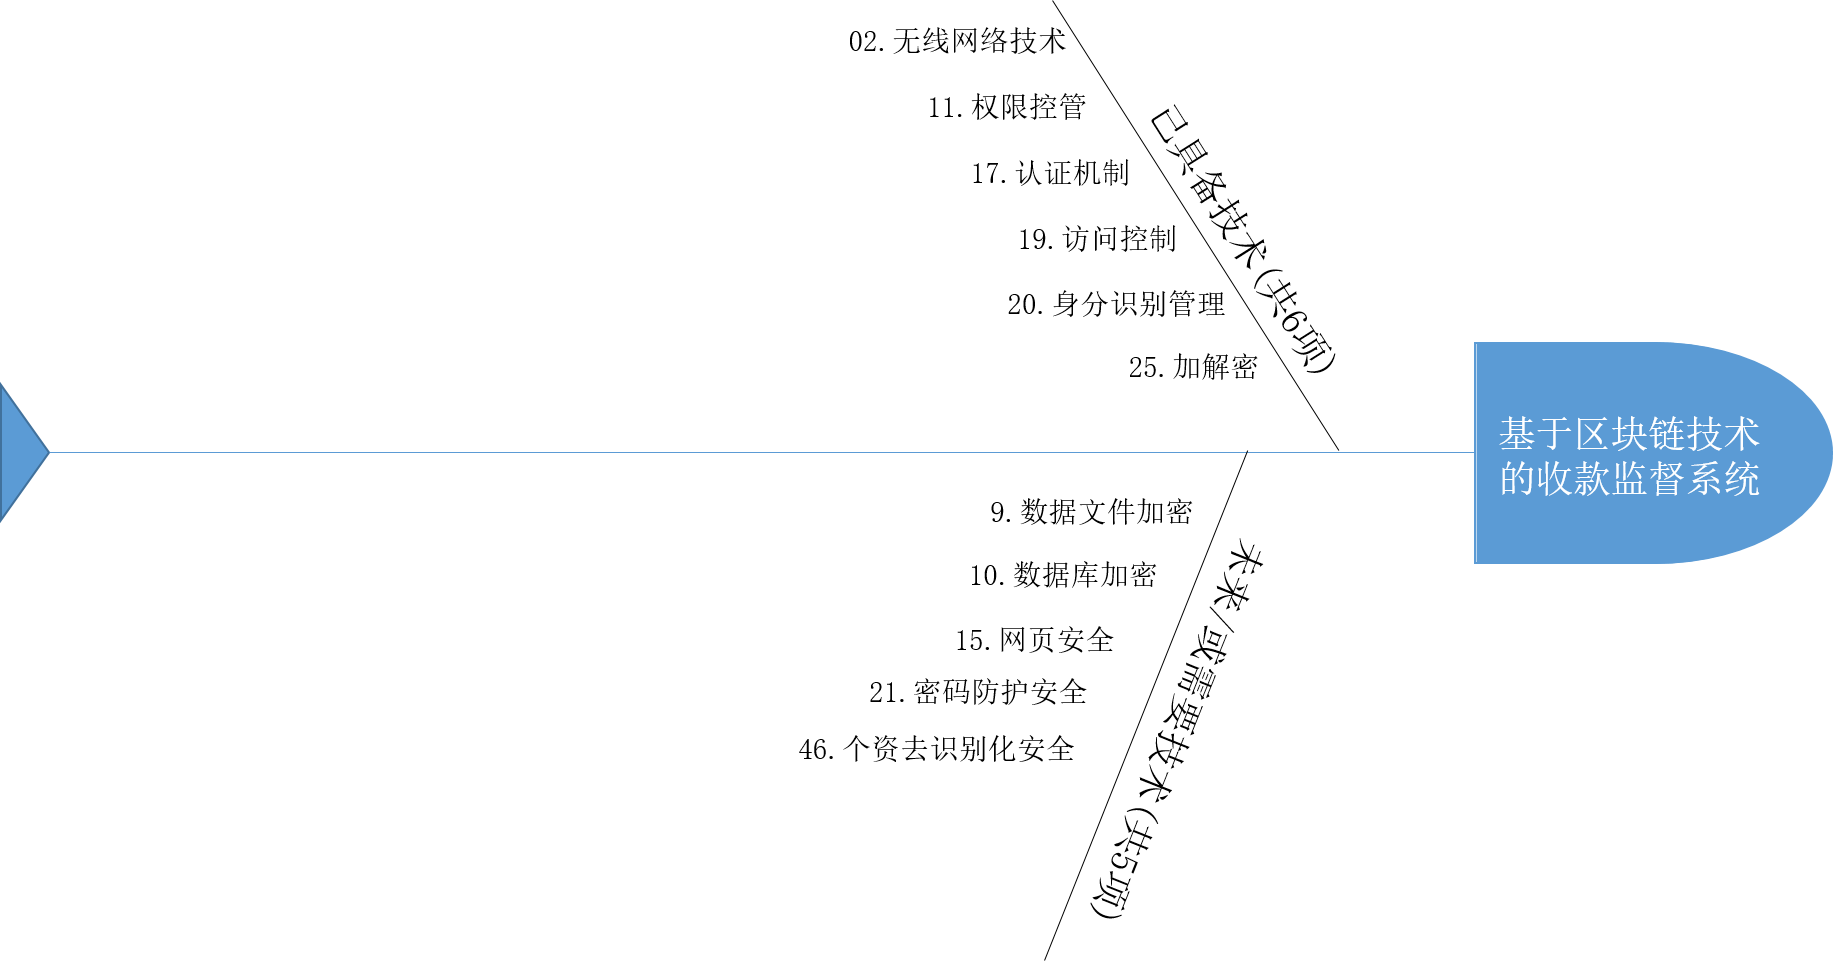
\includegraphics[width = 1\textwidth]{fish2.png}
%			\caption{魚骨圖(2)}\label{fish1}
%		\end{figure}

%		\subsection{匿名顧客對匿名商家}
%	\section{各種交易模型比較}
